%! Author = Len Washington III
%! Date = 11/12/2023

% Preamble
\documentclass[26]{cs430lecture}

% Packages

% Document
\begin{document}

%<*Lecture-Activity-26>
\maketitle
\openingquestions
\begin{enumerate}
    \item What is the difference between a tree and a graph?
    \item Give a recursive definition for a tree.
    \item In a weighted undirected graph, what is the difference between a minimum spanning tree and a shortest path in a graph?
    \item Since the shortest paths contain the shortest sub-paths (\hyperref[dfn:optimal-substructure]{optimal substructure}),
    name an algorithmic approach that we might try to find a shortest path in a graph.
\end{enumerate}

\section{Minimum Spanning Trees}\label{sec:minimum-spanning-trees}
\begin{enumerate}
    \item Give a definition of a Minimum Spanning Tree, and find an MST of the below graph.
    \begin{figure}[H]
        \centering
        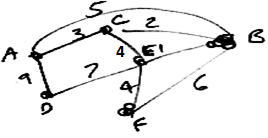
\includegraphics[width=\textwidth]{26.1}
        \label{fig:26.1}
    \end{figure}
    \item Prove a Minimum Spanning Tree has \hyperref[dfn:optimal-substructure]{optimal substructure}.
    \item What are some possible greedy approaches to find a Minimum Spanning Tree?
    Prove correct or show counterexample.
    \item Demonstrate your MST algorithm on the following graph and write pseudocode.
    \begin{figure}[H]
        \centering
        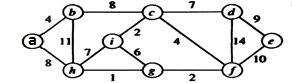
\includegraphics[width=\textwidth]{26.2}
        \label{fig:26.2}
    \end{figure}
\end{enumerate}

Demonstration of Prim (Deleted): \url{http://en.wikipedia.org/wiki/File:Prim-algorithm-animation-2.gif}

Demonstration of Kruskal: \url{https://www.cs.usfca.edu/~galles/visualization/Kruskal.html}
%</Lecture-Activity-26>

\end{document}